\documentclass[10pt]{article}
\usepackage[letterpaper,margin=0.72in,headheight=15pt]{geometry}
\usepackage[T1]{fontenc}
\usepackage{libertinus}
\usepackage{microtype}
\usepackage{amsmath,mathtools}
\usepackage{booktabs,longtable,tabularx,array,multirow}
\usepackage{graphicx}
\usepackage{xcolor}
\usepackage{tikz}
\usetikzlibrary{arrows.meta,positioning,fit}
\usepackage{enumitem}
\usepackage{fancyhdr}
\usepackage{hyperref}
\usepackage{caption}
\usepackage{float}
\usepackage{titlesec}
\usepackage{lastpage}

\definecolor{navy}{HTML}{17324D}
\definecolor{blue}{HTML}{2B6F91}
\definecolor{green}{HTML}{47735A}
\definecolor{amber}{HTML}{A96D1F}
\definecolor{red}{HTML}{A33A32}
\definecolor{ink}{HTML}{1F2A33}
\definecolor{muted}{HTML}{66727D}
\definecolor{line}{HTML}{D7DEE3}
\definecolor{wash}{HTML}{F2F5F6}

\hypersetup{colorlinks=true,linkcolor=navy,urlcolor=blue,citecolor=green,pdfauthor={Jennison Capstone Team},pdftitle={Climate-Finance Scenario, Portfolio and Validation Methodology}}
\pagestyle{fancy}
\fancyhf{}
\lhead{\small\color{navy}\textbf{JENNISON} Climate-Finance Methodology}
\rhead{\small\color{muted}Research prototype}
\cfoot{\small\color{muted}\thepage\ / \pageref{LastPage}}
\renewcommand{\headrulewidth}{0.4pt}
\renewcommand{\headrule}{\hbox to\headwidth{\color{line}\leaders\hrule height \headrulewidth\hfill}}
\titleformat{\section}{\Large\bfseries\color{navy}}{\thesection}{0.6em}{}
\titleformat{\subsection}{\large\bfseries\color{navy}}{\thesubsection}{0.6em}{}
\titleformat{\subsubsection}{\normalsize\bfseries\color{ink}}{\thesubsubsection}{0.6em}{}
\setlist[itemize]{leftmargin=1.3em,itemsep=2pt,topsep=3pt}
\setlist[enumerate]{leftmargin=1.5em,itemsep=3pt,topsep=3pt}
\setlength{\parindent}{0pt}
\setlength{\parskip}{5pt}
\captionsetup{font=small,labelfont=bf,textfont={color=muted}}

\newcommand{\riskbox}[2]{\begin{center}\fcolorbox{line}{wash}{\parbox{0.92\linewidth}{\textbf{\color{navy}#1}\quad #2}}\end{center}}
\newcommand{\impl}{\textcolor{green}{\textbf{Implemented}}}
\newcommand{\proxy}{\textcolor{amber}{\textbf{Calibrated proxy}}}
\newcommand{\gap}{\textcolor{red}{\textbf{Data gap}}}
\newcommand{\R}{\mathbb{R}}

\begin{document}

\begin{titlepage}
\pagecolor{wash}
\vspace*{0.55in}
{\color{navy}\rule{\textwidth}{3pt}}\\[0.35in]
{\fontsize{30}{34}\selectfont\bfseries\color{navy}Climate-Finance Scenario,\\Portfolio and Validation Methodology}\\[0.25in]
{\Large\color{ink}A traceable research architecture for strategic Climate VaR and tactical event risk}\\[0.55in]

\begin{tabularx}{\textwidth}{>{\bfseries\color{navy}}p{1.55in}X}
Prepared for & Jennison client review \\
Version & 21 July 2026 \\
Model scope & U.S.-listed equity and ETF research prototype \\
Primary use & Conditional scenario repricing, portfolio risk budgeting, event overlays, and walk-forward validation \\
\end{tabularx}

\vfill
\riskbox{Central design rule}{Climate information is not assumed to be alpha. It enters strategic allocation through conditional cash-flow loss, scenario penalties, explicit physical and transition budgets, and a separately validated tactical event overlay.}

\vfill
{\small\color{muted}Research prototype only. Not investment advice, a regulatory capital model, a probability forecast, or a substitute for issuer due diligence. The supplied Bloomberg methodology was used as a conceptual reference; no Bloomberg proprietary coefficients or datasets are reproduced.}
\end{titlepage}
\nopagecolor

\setcounter{tocdepth}{1}
\tableofcontents
\newpage

\section{Executive decision summary}

The model is designed to answer four distinct questions without collapsing them into one opaque score:

\begin{enumerate}
  \item \textbf{Strategic value:} how would an issuer or portfolio be valued today if markets repriced from a chosen reference climate path to a target path?
  \item \textbf{Tactical event risk:} which holdings are exposed to today's hazard observations, and what small, funded overlay follows from that exposure?
  \item \textbf{Portfolio construction:} what allocation maximizes a market-derived expected-return proxy while controlling covariance risk and conditional climate losses?
  \item \textbf{Evidence:} does adding climate information improve return, drawdown, or tail behavior relative to the same market-only process?
\end{enumerate}

The architecture follows the strongest elements of scenario-analysis practice: a target-versus-reference comparison, annual cash-flow paths, country-to-sector-to-issuer transmission, firm-specific discount rates, and as-of-date repricing. It extends that structure with a separate NWS event clock, transparent model-risk bands, a robust portfolio objective, and a climate-on versus climate-off validation design.

\riskbox{What the client should focus on}{The most decision-relevant outputs are the scenario-conditioned value impact, the cash-flow attribution by driver, the portfolio's worst conditional scenario loss, the active risk versus the market-only portfolio, and the incremental climate value with uncertainty. A high dashboard score by itself is not an investment conclusion.}

\subsection{What changed in this model revision}

\begin{tabularx}{\textwidth}{p{1.55in}X X}
\toprule
Issue & Previous weakness & Revised treatment \\
\midrule
Transition risk & Atmospheric CO$_2$ could be mistaken for policy pressure & CO$_2$ is context only; transition risk is decomposed into carbon cost, demand, energy cost, transition CapEx, and pass-through \\
GDP transmission & One macro score & Country GDP, sector demand, and supply-chain channels are separate and traceable \\
Physical risk & Alert counts could look like probabilities & Event loss is hazard severity $\times$ location exposure $\times$ vulnerability $\times(1-\text{resilience})$ \\
Time horizon & Recent prices could contaminate long-term climate valuation & Strategic 5--30 year model and tactical 1--20 trading-day overlay are separate clocks \\
Tail metric & Sparse scenarios could be labeled like Expected Shortfall & Conditional scenario range, worst case, and model-ensemble tail are shown; no regulatory ES claim \\
Portfolio & Climate score could be interpreted as unvalidated alpha & Climate enters as loss penalties and risk budgets; expected-return input remains market-derived \\
Backtest & One result could be mistaken for proof & Climate-on versus market-only ablation, costs, bootstrap interval, permutation test, and explicit data limitations \\
\bottomrule
\end{tabularx}

\section{System architecture and two clocks}

\begin{figure}[H]
\centering
\resizebox{\textwidth}{!}{%
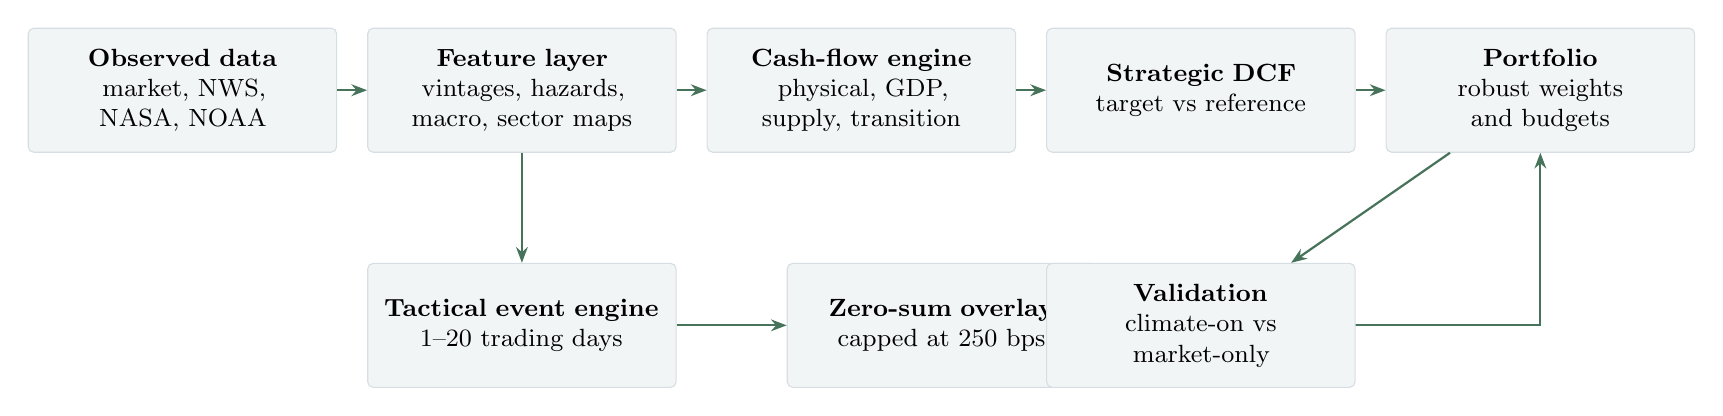
\begin{tikzpicture}[node distance=0.45cm and 0.38cm, every node/.style={font=\small}, box/.style={draw=line,rounded corners=2pt,fill=wash,minimum height=0.62in,text width=1.45in,align=center}, arr/.style={-{Stealth[length=2mm]},thick,color=green}]
\node[box] (data) {\textbf{Observed data}\\market, NWS, NASA, NOAA};
\node[box,right=of data] (features) {\textbf{Feature layer}\\vintages, hazards, macro, sector maps};
\node[box,right=of features] (cash) {\textbf{Cash-flow engine}\\physical, GDP, supply, transition};
\node[box,right=of cash] (dcf) {\textbf{Strategic DCF}\\target vs reference};
\node[box,right=of dcf] (port) {\textbf{Portfolio}\\robust weights and budgets};
\draw[arr] (data)--(features); \draw[arr] (features)--(cash); \draw[arr] (cash)--(dcf); \draw[arr] (dcf)--(port);
\node[box,below=0.55in of features] (event) {\textbf{Tactical event engine}\\1--20 trading days};
\node[box,right=0.55in of event] (overlay) {\textbf{Zero-sum overlay}\\capped at 250 bps};
\draw[arr] (features)--(event); \draw[arr] (event)--(overlay); \draw[arr] (overlay.east)-| (port.south);
\node[box,below=0.55in of dcf] (valid) {\textbf{Validation}\\climate-on vs market-only};
\draw[arr] (port)--(valid);
\end{tikzpicture}
}
\caption{Closed-loop architecture. Strategic valuation and tactical event response share source lineage but do not share a time clock.}
\end{figure}

The final weight is
\begin{equation}
w_t = w_t^{\mathrm{Strategic}} + \Delta w_t^{\mathrm{Event}},
\qquad
\mathbf{1}^{\top}\Delta w_t^{\mathrm{Event}}=0,
\qquad
|\Delta w_{i,t}^{\mathrm{Event}}|\le 250\ \text{bps}.
\end{equation}
The strategic model uses annual scenario paths and one-year daily market history for covariance and the market return proxy. Current NWS alerts do not alter strategic weights. The event overlay can update daily, but it must fund itself, respect position and sector caps, and remain small relative to the strategic allocation.

\section{Data architecture and lineage}

\subsection{Observed, calibrated, and missing}

\begin{longtable}{p{1.10in}p{1.05in}p{0.95in}p{3.10in}}
\toprule
Source & Model role & Current status & Control and interpretation \\
\midrule
\endhead
NWS active alerts & Tactical acute hazard severity & \impl & Used as a current event nowcast, never as a long-run disaster probability \\
NASA GISTEMP & Chronic climate state & \impl & Current warming context and chronic-risk calibration \\
NOAA/NCEI disasters & Historical physical-loss context & \impl & Disaster frequency and loss history; not an issuer damage estimate \\
NOAA GML CO$_2$ & Climate-state context & \impl & Displayed for context and excluded from transition risk \\
NGFS scenario paths & GDP, inflation, energy, carbon, physical pathways & \proxy & Transparent scenario calibrations are operational; production-grade annual ingestion and version pinning remain required \\
BEA GDP by Industry & Sector value added and GDP sensitivity & \proxy & Model contains a BEA-style sector mapping; direct production ingestion remains source-ready \\
BEA Input-Output & Direct and indirect supply-chain transmission & \proxy & Supply beta is explicit; full requirements-table ingestion remains source-ready \\
FRED/ALFRED & Point-in-time macro vintages & \gap & Required before macro backtests can be called fully point-in-time \\
EIA and EPA eGRID & Energy price, generation mix, emissions intensity & \proxy & Sector calibrations are explicit; issuer/facility joins remain source-ready \\
SEC XBRL & Revenue, cost, CapEx, capital structure & \proxy & WACC uses market beta and sector capital-structure fallback; direct issuer ingestion remains source-ready \\
Facility coordinates & Bottom-up hazard exposure & \gap & A documented issuer-facility schema exists; absent records are labeled as sector fallback \\
Supplier/customer graph & Indirect transition and interruption risk & \gap & Needed for issuer-level second-order exposure \\
\bottomrule
\end{longtable}

Official sources are chosen because they support traceability. BEA requirements tables describe both direct and indirect inputs across industries; ALFRED exposes historical vintages; NASA NEX-GDDP-CMIP6 provides bias-corrected downscaled daily projections; EPA eGRID describes power-sector emissions and resource mix; EIA provides energy prices and generation data; and SEC APIs provide machine-readable filings. These sources improve auditability but do not remove model risk.

\subsection{Point-in-time rule}

For a signal formed at date $t$, every feature must satisfy
\begin{equation}
\mathrm{availability\_date}(x) \le t.
\end{equation}
Annual climate features use the latest completed calendar-year vintage and expanding-window normalization. Market features use observations strictly prior to the next-day return. Production validation additionally requires historical index membership, delisted securities, filing timestamps, archived NWS/NOAA observations, and ALFRED macro vintages.

\section{Strategic model: scenario to firm value}

\subsection{Target versus reference}

Let $s$ denote the target scenario and $r$ the reference. The model evaluates the immediate, as-of-date valuation change implied by replacing the reference path with the target path. It does not assign a probability to either path:
\begin{equation}
\Delta X_{s,t}=X_{s,t}-X_{r,t}.
\end{equation}
This aligns with the scenario-conditioned repricing principle in the supplied Bloomberg methodology. It is a sensitivity analysis, not a forecast.

\subsection{Country GDP, sector demand, and supply chain}

The revenue-growth channel is decomposed rather than hidden inside one macro score:
\begin{equation}
\Delta g^{\mathrm{Revenue}}_{i,s,t}
=\beta^{GDP}_{i}\Delta GDP_{c,s,t}
+\beta^{Demand}_{i}\Delta Demand_{k,s,t}
+\beta^{Supply}_{i}\Delta SupplyFactor_{s,t}.
\end{equation}
The implementation uses a country path, BEA-style sector GDP and input-output betas, and an issuer earnings-sensitivity fallback. Revenue geography and actual supplier/customer weights are explicitly marked missing when they are unavailable. Country, sector, and supply-chain terms remain separate in both the DCF and the Shapley attribution, preventing the same demand effect from being counted twice.

\subsection{Transition cash-flow channels}

Atmospheric CO$_2$ concentration is a climate-state observation, not a policy instrument. Transition risk is therefore defined through financially interpretable channels:
\begin{align}
TR_{i,s,t}={}&CarbonCost_{i,s,t}+DemandShift_{i,s,t}+EnergyCost_{i,s,t}\nonumber\\
&+TransitionCapex_{i,s,t}-PassThrough_{i,s,t}.
\end{align}
Each term maps to an issuer cash-flow line:
\begin{itemize}
  \item $CarbonCost$: emissions intensity $\times$ scenario carbon-price shock;
  \item $DemandShift$: product/sector demand path $\times$ demand elasticity;
  \item $EnergyCost$: energy intensity $\times$ scenario energy-price shock;
  \item $TransitionCapex$: required investment intensity $\times$ scenario adjustment path;
  \item $PassThrough$: the share of carbon and energy costs recoverable through prices.
\end{itemize}
Positive values reduce FCFF; pass-through is recorded as a negative loss. Current sector coefficients are disclosed fallbacks until issuer-level NGFS, EIA, eGRID, and SEC joins are loaded.

\subsection{Top-down physical risk}

Country physical losses are conserved when downscaled to sectors. For risk type $q\in\{\mathrm{acute},\mathrm{chronic}\}$,
\begin{equation}
\Delta Y^{q}_{j,t}=\frac{\alpha^{q}_{j}}{\sum_k \omega_k\alpha^{q}_{k}}\Delta Y^{q}_{c,t},
\end{equation}
where $\omega_k$ is sector $k$'s value-added share. The weighted sector multiplier reconciles to one. Firm-level differentiation is bounded:
\begin{equation}
\Delta Y^{q}_{i,j,t}=
\mathrm{clip}\!\left(\frac{\alpha^{q}_{i,j}}{\widetilde{\alpha}^{q}_{j}},a_{\min},a_{\max}\right)
\Delta Y^{q}_{j,t}.
\end{equation}
Fixed-asset intensity proxies acute vulnerability and labor intensity proxies chronic vulnerability. Missing issuer observations use labeled sector medians.

\subsection{Bottom-up event loss}

The tactical physical engine uses a different equation:
\begin{equation}
Loss_{i,h,t}=Hazard_{h,l,t}\times Exposure_{i,l}\times Vulnerability_{i,h}\times(1-Resilience_i).
\end{equation}
NWS contributes current severity and hazard mix. Location exposure should come from facilities, employees, insured assets, and critical suppliers. Vulnerability is peril and asset-type specific. Resilience includes insurance, backup capacity, supplier substitution, and adaptation investment. When facility data are absent, the interface says ``sector hazard fallback'' rather than implying asset-level precision.

\subsection{Climate-adjusted FCFF and DCF}

The modeled free cash flow is
\begin{align}
FCFF_{i,s,t}={}&Revenue_{i,s,t}-OperatingCost_{i,s,t}-CarbonCost_{i,s,t}\nonumber\\
&-Damage_{i,s,t}-AdaptationCapex_{i,s,t}.
\end{align}
The engine applies nonlinear annual paths: orderly transition effects arrive earlier, delayed-transition effects arrive later, and physical losses accelerate toward the horizon. Firm value is
\begin{equation}
V_{i,s}=\sum_{t=1}^{T}\frac{FCFF_{i,s,t}}{(1+WACC_i)^t}
+\frac{FCFF_{i,s,T}(1+g_{i,s})}{(WACC_i-g_{i,s})(1+WACC_i)^T}.
\end{equation}
The discount rate is issuer-specific where market beta is observable and otherwise uses a sector fallback:
\begin{equation}
WACC_i=\frac{E}{V}(r_f+\beta_i ERP)+\frac{D}{V}r_d(1-\tau_c).
\end{equation}
The prototype uses disclosed risk-free, equity-risk-premium, debt-cost, tax, leverage, and terminal-growth assumptions. A production model should source debt and capital structure directly from filings and market data.

\subsection{Conditional Climate VaR and attribution}

For each scenario,
\begin{equation}
ClimateVaR_{i,s}=\frac{V_{i,r}-V_{i,s}}{V_{i,r}}.
\end{equation}
The model reports each conditional loss, the cross-scenario range, the worst conditional loss, and the mean of the two largest losses as a \emph{model-ensemble tail proxy}. With five stress scenarios and no defensible occurrence probabilities, this proxy is not 95\% Expected Shortfall.

Attribution uses exact Shapley values over nine DCF channels: acute physical, chronic physical, country GDP, sector demand, supply chain, carbon cost, energy cost, transition CapEx, and pass-through. The implementation checks that contributions reconcile to total value impact, with a residual near zero.

\section{Model-risk sensitivity}

The physical loss function is uncertain even when scenario data are official. The platform reruns every scenario with physical damage coefficients scaled to $0.70\times$ and $1.30\times$:
\begin{equation}
\mathcal{B}^{phys}_{s}=\left[ClimateVaR_s(0.70\alpha^{phys}),\ ClimateVaR_s(1.30\alpha^{phys})\right].
\end{equation}
This is a transparent sensitivity band, not a confidence interval. It is especially important because NGFS states that the academic paper underpinning parts of Phase V physical-loss estimates was retracted and that an updated methodology is expected in the next long-term scenario release. Therefore, NGFS is treated as one scenario input, not as ground truth.

Future production sensitivity should add alternative damage functions, climate-model ensembles, hazard return periods, adaptation assumptions, WACC shocks, carbon-price paths, demand elasticities, and pass-through ranges.

\section{Portfolio construction}

\subsection{Market return proxy and covariance}

The expected-return proxy $\mu$ is derived from market information only: 12-month momentum, liquidity, recent return, and volatility control. Climate variables do not receive an assumed return premium. The covariance matrix $\Sigma$ uses up to 252 aligned daily returns and is annualized; a diagonal variance fallback is labeled when pairwise history is insufficient.

\subsection{Robust objective}

Within ETF and stock sleeves, the strategic allocation solves the projected-gradient problem
\begin{align}
\max_{w}\quad
&\mu^\top w-\lambda w^\top\Sigma w
-\kappa\max_{s\in\mathcal{S}}L_s(w)\nonumber\\
&-\eta(w-w^{mkt})^\top\Sigma(w-w^{mkt})
-\tau\lVert w-w^{mkt}\rVert_1,
\end{align}
where
\begin{equation}
L_s(w)=\sum_i w_i\ell_{i,s}.
\end{equation}
At each iteration the solver identifies
\begin{equation}
s^*=\arg\max_s L_s(w)
\end{equation}
and uses the loss vector $\ell_{\cdot,s^*}$ as a subgradient. This is materially different from adding each security's independent worst loss, which can overstate or misstate portfolio stress.

The feasible set includes:
\begin{align*}
&\mathbf{1}^\top w=1,\quad 0\le w_i\le \bar w_i,\quad \sum_{i\in sector\ j}w_i\le 35\%,\\
&\max_s L_s(w)\le B_{scenario},\quad w^\top p\le B_{physical},\quad w^\top q\le B_{transition},\\
&w^\top c\le B_{carbon},\quad TE(w,w^{mkt})\le B_{TE}.
\end{align*}
If the selected universe makes a budget infeasible, the result is marked \textbf{Watch}; it is not silently reported as a pass. Broad-market ETFs are modeled as an economy composite rather than defaulting to Technology.

\subsection{Tactical overlay}

For short-horizon mode, a centered score combines market confirmation and event loss:
\begin{equation}
z_{i,t}=0.55(M_{i,t}-0.5)-0.45E_{i,t},\qquad
\widetilde z_{i,t}=z_{i,t}-\frac{1}{N}\sum_jz_{j,t}.
\end{equation}
The overlay is scaled, capped at 250 bps, projected back to each sleeve budget, and then rechecked against position and sector constraints. Long-horizon mode sets this overlay to zero.

\begin{figure}[H]
\centering
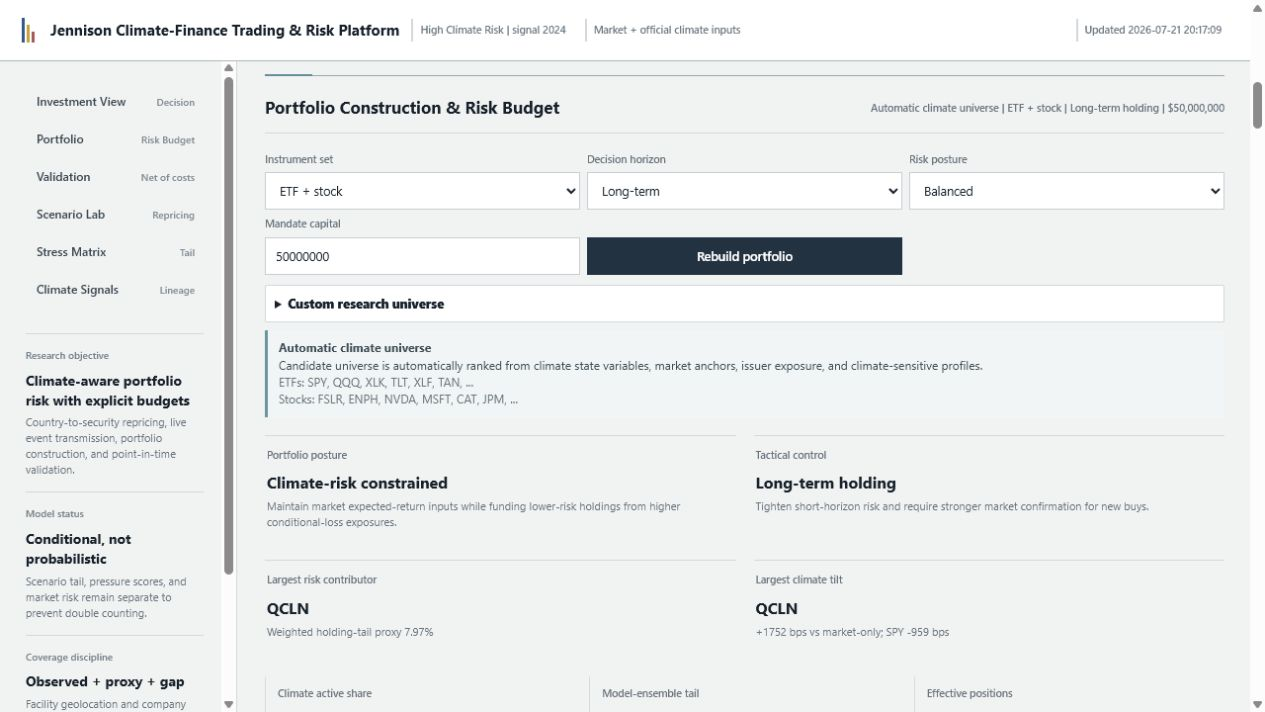
\includegraphics[width=\textwidth]{figures/portfolio-risk-budget.png}
\caption{Portfolio Construction and Risk Budget. The interface separates the strategic portfolio, market-only reference, active climate-risk weight, and each feasibility check. Values are an illustrative live run and will change with market data.}
\end{figure}

\section{Walk-forward validation}

\subsection{Signal timing and execution}

For each signal date $t$, the model forms buy and sell books using only information available through $t$, then applies the position to $t+1$ returns. Reported net return is
\begin{equation}
r^{net}_{t+1}=r^{gross}_{t+1}-Turnover_t\times Cost_{trade}-ShortExposure_t\times\frac{Cost_{borrow}}{252}.
\end{equation}
The benchmark uses the same net risky exposure and cash weight. The three-week window is a monitoring diagnostic; three months is tactical evidence; three years provides broader context but remains conditional on the available universe history.

\subsection{Climate-on versus market-only ablation}

The central validation estimand is
\begin{equation}
IncrementalClimateValue=
Wealth_{FullModel}-Wealth_{MarketOnly},
\end{equation}
where both books use the same assets, gross/net exposure, transaction costs, borrow costs, and next-day execution. This design asks whether climate information adds value beyond ordinary market selection rather than comparing unrelated portfolios.

Uncertainty is reported with a five-day moving-block bootstrap and a two-sided sign-permutation test on daily incremental returns. The platform does not call an effect statistically significant merely because total return is positive.

\begin{figure}[H]
\centering
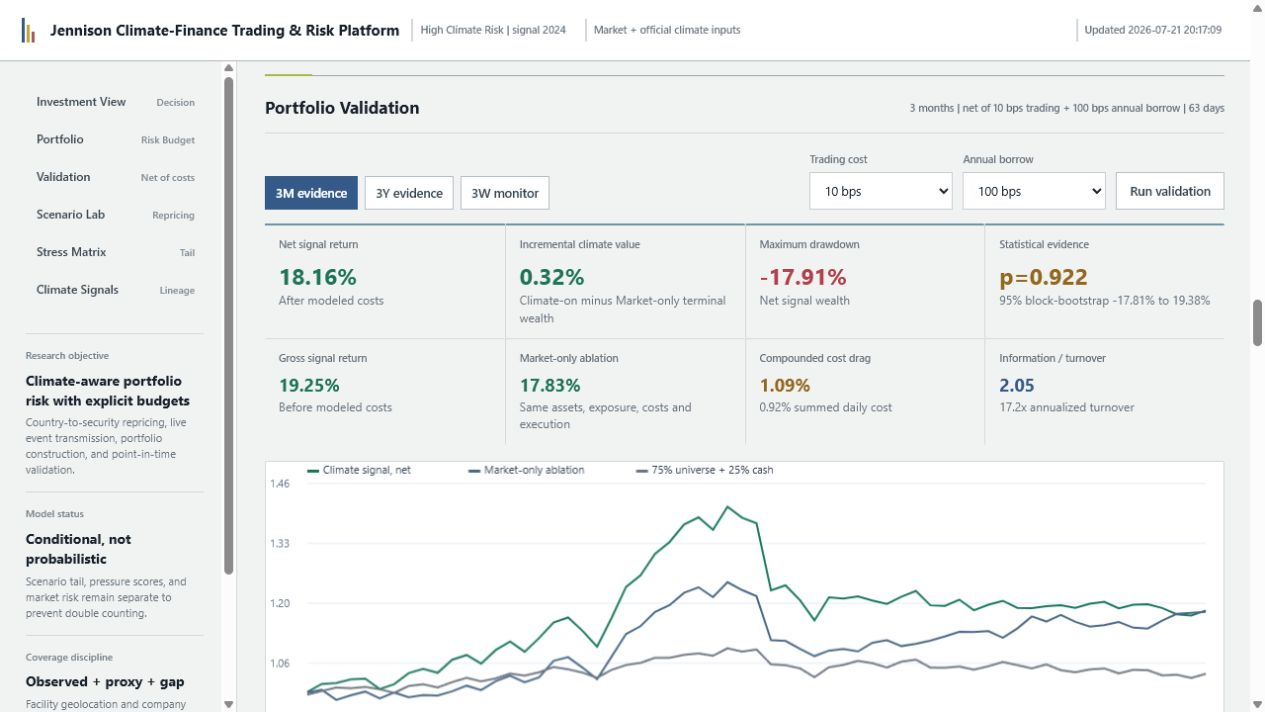
\includegraphics[width=\textwidth]{figures/walk-forward-validation.png}
\caption{Three-month validation captured on 21 July 2026. In this run the incremental climate value was small and statistically inconclusive; the interface reports the result rather than hiding it.}
\end{figure}

\subsection{Current validation boundary}

The present replay is useful for system diagnostics but is not yet production performance evidence. It does not reconstruct a complete archived NWS tape, historical index constituents, delisted securities, ALFRED macro vintages, security-level locate constraints, market impact, financing, or taxes. Until those are loaded, claims should be limited to conditional research evidence.

\section{Reading the Scenario and Event Lab}

\begin{figure}[H]
\centering
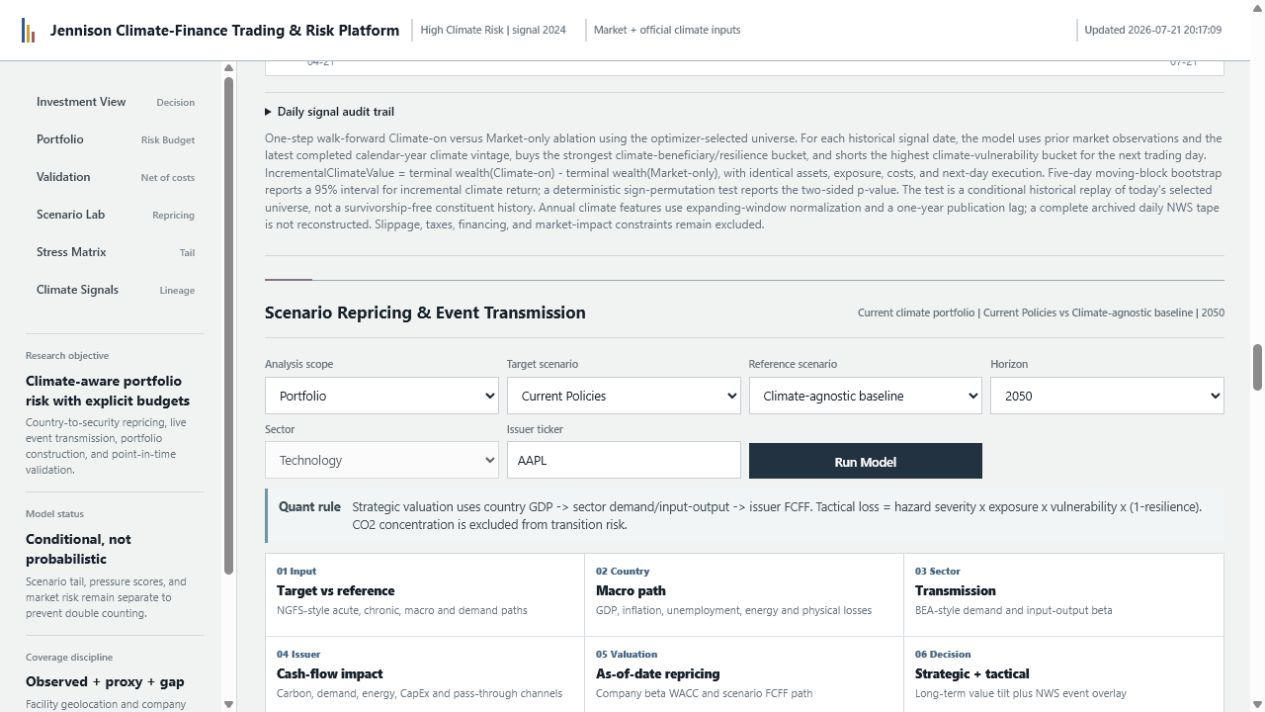
\includegraphics[width=\textwidth]{figures/scenario-event-lab.png}
\caption{Scenario and Event Lab. Long-term DCF attribution and short-term hazard transmission are displayed together but calculated separately.}
\end{figure}

The client should read the page in this order:
\begin{enumerate}
  \item Confirm the target, reference, horizon, and scope.
  \item Read total value impact as a conditional as-of-date revaluation, not a probability-weighted forecast.
  \item Identify whether acute, chronic, GDP, supply, or transition channels explain the result.
  \item Check WACC, terminal growth, issuer fallback quality, and attribution residual.
  \item Read NWS event risk separately and confirm that a tactical overlay is zero-sum and capped.
  \item Compare the scenario result with the model-risk sensitivity band before making a risk-budget decision.
\end{enumerate}

\section{Bloomberg alignment and deliberate differences}

The supplied Bloomberg paper describes an obligor-centric, target-versus-reference, as-of-date repricing framework that transmits micro transition, macro transition, acute physical, and chronic physical effects into cash flow and then firm value. It also emphasizes detailed revenue segmentation, supply-chain links, firm-specific WACC, and separate equity/debt allocation.

This prototype adopts the following public and reproducible logic:
\begin{itemize}
  \item target and reference scenario comparison;
  \item annual scenario-conditioned cash-flow paths;
  \item country GDP to sector and issuer transmission;
  \item separate acute/chronic and micro/macro channels;
  \item as-of-date DCF using firm/sector-specific WACC;
  \item portfolio aggregation and contribution analysis;
  \item explicit data-quality fallbacks.
\end{itemize}

The prototype deliberately does not claim to reproduce Bloomberg proprietary inputs, TRACT revenue projections, supply-chain data, DRSK default probabilities, Merton-Black-Cox equity/debt allocation, or bond OAS repricing. Its differentiating features are open traceability, a separate real-time event clock, robust portfolio constraints, climate-on/off ablation, and explicit disclosure of unavailable inputs.

\section{Controls, tests, and governance}

The codebase includes 26 automated methodology tests. Core controls include:
\begin{itemize}
  \item target equals reference implies zero value impact;
  \item physical sector downscaling conserves country loss;
  \item CO$_2$ changes do not change transition risk;
  \item transition and GDP components are counted once;
  \item Shapley contributions reconcile to total value impact;
  \item NWS overlay is zero-sum and capped, and no hazard mix means no trade;
  \item missing facility data is labeled as sector fallback;
  \item portfolio weights, caps, HHI, and risk checks reconcile;
  \item broad-market ETFs use an economy composite;
  \item market history is never replaced with simulated returns;
  \item walk-forward return includes modeled turnover and costs.
\end{itemize}

Model governance should add versioned parameter files, maker-checker approval for calibration changes, source-file hashes, data-vintage manifests, exception logs, challenger models, and periodic performance decay reviews.

\section{Production roadmap}

\begin{longtable}{p{0.40in}p{1.25in}p{3.25in}p{1.25in}}
\toprule
Rank & Workstream & Acceptance criterion & Primary source \\
\midrule
\endhead
1 & Point-in-time data store & Every backtest feature has an availability timestamp; archived NWS/NOAA and ALFRED vintages are reproducible & NWS, NOAA, ALFRED \\
2 & Scenario ingestion & Version-pinned annual NGFS variables with unit, model, region, and release metadata & NGFS \\
3 & Macro and supply-chain calibration & BEA GDP-by-industry and requirements tables replace hand-set sector betas & BEA \\
4 & Issuer financials & Revenue, margin, CapEx, debt, tax, and segment data joined by filing date & SEC XBRL \\
5 & Energy transition & Carbon intensity, generation mix, and energy-price channels are issuer/facility specific & EIA, EPA eGRID \\
6 & Physical geolocation & Facilities and critical suppliers mapped to peril layers with validated vulnerability curves & NASA, FEMA, NOAA \\
7 & Portfolio implementation & Prior holdings, turnover, ADV capacity, market impact, borrow, and mandate constraints & Client + market data \\
8 & Independent validation & Challenger damage functions, bootstrap stability, attribution, and model-risk committee sign-off & Internal governance \\
\bottomrule
\end{longtable}

\section{Conclusion}

The revised model no longer asks a client to trust an abstract climate score. It produces a chain that can be challenged at every step:
\begin{center}
\textbf{source and vintage $\rightarrow$ economic channel $\rightarrow$ FCFF path $\rightarrow$ DCF loss $\rightarrow$ portfolio constraint $\rightarrow$ validated action.}
\end{center}

The strongest current capability is transparent conditional scenario analysis joined to an auditable portfolio and validation layer. The largest remaining limitation is data granularity: full value will require point-in-time macro vintages, issuer financials, facility locations, product revenue, and supplier/customer links. The correct next step is deeper evidence, not another composite score.

\appendix
\section{Parameter and formula ledger}

\begin{tabularx}{\textwidth}{p{1.55in}X p{1.25in}}
\toprule
Item & Implemented rule & Governance status \\
\midrule
Strategic horizon & Annual paths to 2030, 2040, or 2050 & User-selectable \\
Tactical horizon & 1--20 trading days & Separate clock \\
Physical path shape & $progress^{1.35}$ & Sensitivity required \\
Transition path shape & Orderly $0.70$; delayed $2.10$; hot house $1.20$; fragmented $1.55$ & Disclosed calibration \\
Risk-free rate & 4.25\% & Replace with as-of-date curve \\
Equity risk premium & 4.50\% & Governance input \\
Pre-tax debt cost & 5.25\% & Replace with issuer spread \\
Corporate tax rate & 21\% & U.S. fallback \\
Single-name cap & 20\% maximum effective cap & Internal threshold \\
Sector cap & 35\% & Hard transfer check \\
Event overlay & 250 bps per security, zero-sum & Hard cap \\
Scenario probability & None assigned & Conditional stresses \\
Tail proxy & Mean of two largest conditional losses & Not Expected Shortfall \\
Physical model risk & 0.70--1.30 damage multiplier & Sensitivity, not CI \\
\bottomrule
\end{tabularx}

\section{Notation}
\begin{tabularx}{\textwidth}{p{0.75in}X p{0.75in}X}
\toprule
Symbol & Meaning & Symbol & Meaning \\
\midrule
$i$ & issuer or instrument & $j$ & sector \\
$c$ & country & $s$ & climate scenario \\
$h$ & physical hazard & $t$ & time \\
$w$ & portfolio weight vector & $\Sigma$ & annualized return covariance \\
$\mu$ & market-derived expected-return proxy & $L_s(w)$ & conditional portfolio loss \\
$V_{i,s}$ & issuer value under scenario & $WACC_i$ & issuer discount rate \\
\bottomrule
\end{tabularx}

\section{References and source notes}

\begin{thebibliography}{9}
\bibitem{bloomberg2026} Bloomberg L.P. (2026). \emph{Bloomberg Climate Scenario Analysis for Corporate Securities}. Supplied client reference; confidential/proprietary source reviewed for conceptual alignment only.
\bibitem{ngfs5} Network for Greening the Financial System. \emph{NGFS Climate Scenarios for central banks and supervisors -- Phase V}. Notice updated February 2026. \url{https://www.ngfs.net/en/publications-and-statistics/publications/ngfs-climate-scenarios-central-banks-and-supervisors-phase-v}
\bibitem{beaIO} U.S. Bureau of Economic Analysis. \emph{Input-Output Accounts}. \url{https://www.bea.gov/data/industries/input-output-accounts-data}
\bibitem{beaGDP} U.S. Bureau of Economic Analysis. \emph{GDP by Industry}. \url{https://www.bea.gov/data/gdp/gdp-industry}
\bibitem{alfred} Federal Reserve Bank of St. Louis. \emph{FRED and ALFRED API}. \url{https://fred.stlouisfed.org/docs/api/fred/overview.html}
\bibitem{nasa} NASA Center for Climate Simulation. \emph{NEX-GDDP-CMIP6}. \url{https://www.nccs.nasa.gov/data-collections/nex-gddp-cmip6/}
\bibitem{egrid} U.S. Environmental Protection Agency. \emph{Emissions \& Generation Resource Integrated Database}. \url{https://www.epa.gov/egrid}
\bibitem{eia} U.S. Energy Information Administration. \emph{Open Data API}. \url{https://www.eia.gov/opendata/}
\bibitem{sec} U.S. Securities and Exchange Commission. \emph{EDGAR Application Programming Interfaces}. \url{https://www.sec.gov/search-filings/edgar-application-programming-interfaces}
\bibitem{nws} National Weather Service. \emph{Alerts Web Service}. \url{https://www.weather.gov/documentation/services-web-alerts}
\end{thebibliography}

\vfill
{\small\color{muted}\textbf{Document control.} Generated from the same repository that contains the calculation engine, automated tests, interface, and report figures. Numeric screenshots are illustrative snapshots and are not guaranteed to reproduce after source data refresh.}

\end{document}
